\subsection{Height Tab}

Per default, a target reports height is not used for display, which is common in current air-traffic displays. However, in certain situation a true 3D display might be of interest to a user, and therefore several options where incorporated:

%  \item Use Height: Whether height information should be used to create a 3D presentation
%  \item Offset Factor: If height information is used, this factor is added to the height
%  \item Scale Factor: If height information is used, this factor is used to multiply the height
%  \item Null Offset: If height information is used, this factor is used for target reports without height information


\begin{itemize}
 \item Use Height: Use the height based on Mode C $h_c$, transformed to meters
 \item Offset Factor: If height information is used, this factor $h_o$ is added to the height
 \item Scale Factor: If height information is used, this factor $h_s$ is used to multiply the height
 \item Null Offset: If height information is used, this factor $h_n$ is used for target reports without height information
\end{itemize}

Generally, if no height information is given (no Mode C code), the height is either $0$ or the height offset (if used). That means that those target reports appear to the on the ground. If connection lines are drawn between the ones in the air and those without, a lot of annoying lines are shown.

The formula to calculate the height (if existing) is as follows:

$$ h = h_o + h_s \cdot h_c [m]$$ 

If no height information is given:

$$ h = h_n [m]$$ 

Please note that upon changes to the height usage, a manual redraw has to be performed using the 'Redraw' button.


\begin{figure}[H]
    \hspace*{-2.5cm}
    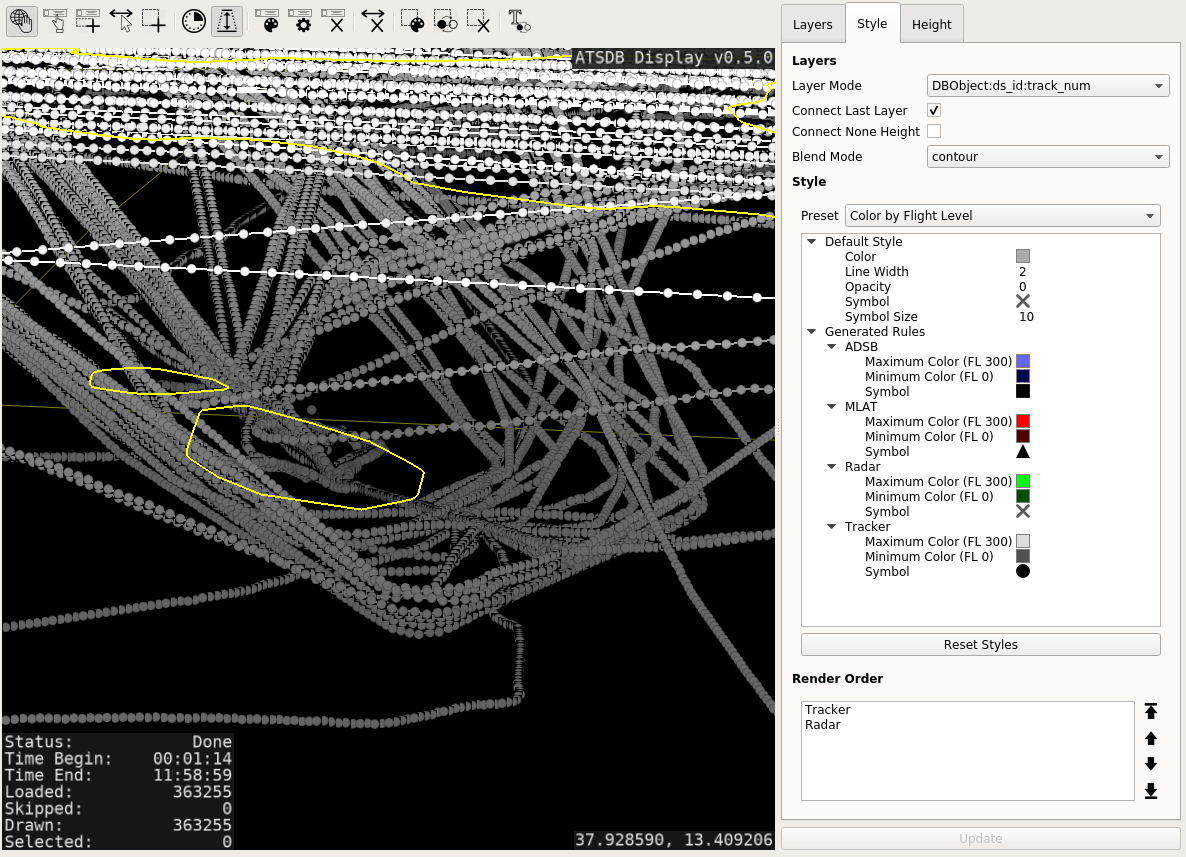
\includegraphics[width=19cm,frame]{../screenshots/osgview_use_height.png}
  \caption{OSG View use height}
\end{figure} 
